\documentclass[border=2pt]{standalone}
\usepackage{tikz}
\usetikzlibrary{arrows.meta,calc,shapes.arrows}
\begin{document}
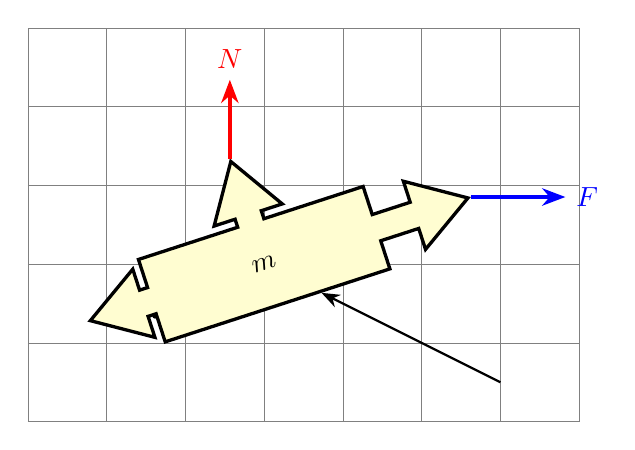
\begin{tikzpicture}[>=Stealth]
  \draw[help lines] (-3,-2) grid (4,3);
  \node[arrow box,draw,very thick,fill=yellow!18,rotate=18,
    minimum width=30mm,minimum height=11mm,
    arrow box arrows={east:12mm,west:8mm,north:8mm},
    arrow box shaft width=3.5mm,arrow box head extend=2.8mm,
    arrow box tip angle=65] (body) at (0,0) {$m$};
  \draw[->,very thick,blue] (body.east arrow tip) -- ++(1.2,0) node[right] {$F$};
  \draw[->,very thick,red] (body.north arrow tip) -- ++(0,1) node[above] {$N$};
  \draw[->,thick] (3,-1.5) -- (body);
  \fill[black] (body.before west arrow) circle (1pt);
\end{tikzpicture}
\end{document}
